\documentclass{beamer}
\usepackage{fontspec,xunicode,xltxtra,beamerthemesplit}
\usepackage{graphicx}
\usepackage{beamerthemeshadow}
%\usepackage{algorithmic}
%\usepackage{algorithm}
\usepackage[CJKmath = true]{xeCJK}
\usepackage{fancyhdr}

\usetheme{Antibes}
%\setsansfont[Mapping=tex-text]{SimSun}
%\setmainfont[BoldFont=Microsoft YaHei]{SimSun}
%\setmonofont{Microsoft YaHei}
\setCJKmainfont[BoldFont=Microsoft YaHei]{SimSun}
%\setCJKmainfont{SimSun}
%\setCJKmathfont{楷体}
%\setCJKsansfont{Times New Roman}


\title{相关问题检索}
\author{赵惜墨}
\date{\today}
\institute{哈尔滨工业大学\\计算机学院\\智能技术与自然语言处理实验室}

\XeTeXlinebreaklocale "zh" % 表示用中文的断行
\XeTeXlinebreakskip = 0pt plus 1pt % 多一点调整的空间

\begin{document}



\frame{\titlepage}

\section{方法概述}

\frame{
  \frametitle{例子}

  \begin{figure}
  \centering
  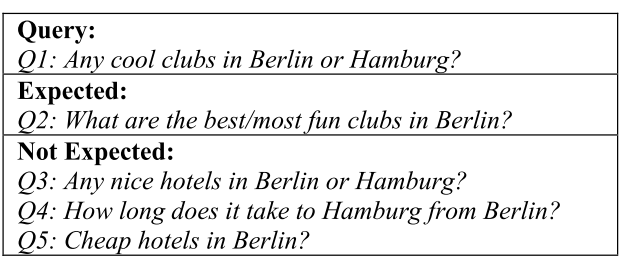
\includegraphics[height=3cm,width=6cm]{querysearch.png}
  \caption{问句检索相关例子}
  \label{fig:vsm}
  \end{figure}

}

\frame{
  \frametitle{基本方法}

  \begin{itemize}
  \item VSM(vector space model)
  \item LM(language model)
  \item Translation Model(the state of the art)
  \end{itemize}

}

\frame{
  \frametitle{这周看的}

  \begin{itemize}
  \item Cao et al., 2010 提出了一个识别cQA中通用问题的框架,将问句匹配分为全局匹配和局部匹配两个子问题,从而提升了结果。
  \item Duan et al., 2008 提出了一种基于MDL(最小描述距离)的方法,将问句转化为对于question topic 和question focus两个子问题的匹配方法。
  \item Cai et al., 2011 提出了将LDA和问句匹配相联合的方法。
  \end{itemize}

}

\section{基本方法简述}

\subsection{VSM}

\frame{
  \frametitle{VSM model}

  \begin{figure}
  \centering
  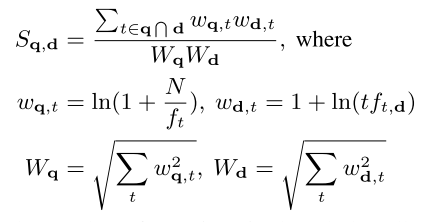
\includegraphics[height=3cm,width=5cm]{vsm.png}
  \caption{VSM model}
  \label{fig:vsm}
  \end{figure}
}

\subsection{Okapi BM25}

\frame{
  \frametitle{Okapi BM25 Model}

  \begin{figure}
  \centering
  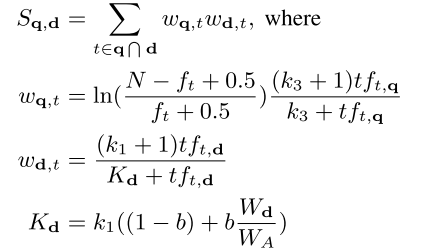
\includegraphics[height=3cm,width=5cm]{bm25.png}
  \caption{Okapi BM25 Model}
  \label{fig:bm25}
  \end{figure}

  解决了VSM偏向于选择短问题的问题。
}

\subsection{LM}

\frame{
  \frametitle{Language Model}

  \begin{figure}
  \centering
  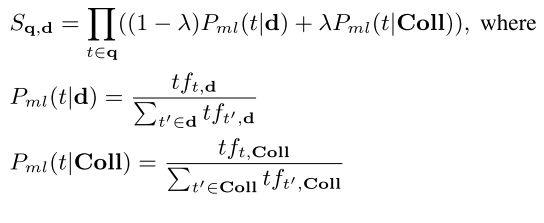
\includegraphics[height=3cm,width=7cm]{lm.png}
  \caption{Language Model}
  \label{fig:lm}
  \end{figure}
  
}

\section{Category Enhanced Retrieval Model}

\frame{
  \frametitle{Category Enhanced Retrieval Model}

  目标函数
  \begin{displaymath}
    RS_{q,d} = (1-\alpha ) N(S_{q,d}) + \alpha N(S_{q,cat(d)})
  \end{displaymath}
  
}

\subsection{Global Relevance}

\frame{
  \frametitle{Global Relevance}
  
  \begin{itemize}
  \item 一种非常naive的idea是直接将类别的词作为一个大的文章进行计算
  \item 由于类别间的词表长度差异非常大(467-69789),这样做会直接导致归一化系数占主导地位
  \end{itemize}
  \begin{figure}
  \centering
  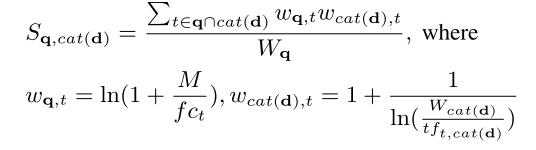
\includegraphics[height=2cm,width=6cm]{gr.png}
  \caption{Global Relevance for VSM}
  \label{fig:gr}
  \end{figure}

  其他模型也做了类似的调整。

}

\subsection{Local Relevance}

\frame{
  \frametitle{Local Relevance}

  对于局部匹配,只根据类别内部计算IDF。
}

\subsection{Result Analysis}

\frame{
  \frametitle{Result Analysis}

  \begin{figure}
  \centering
  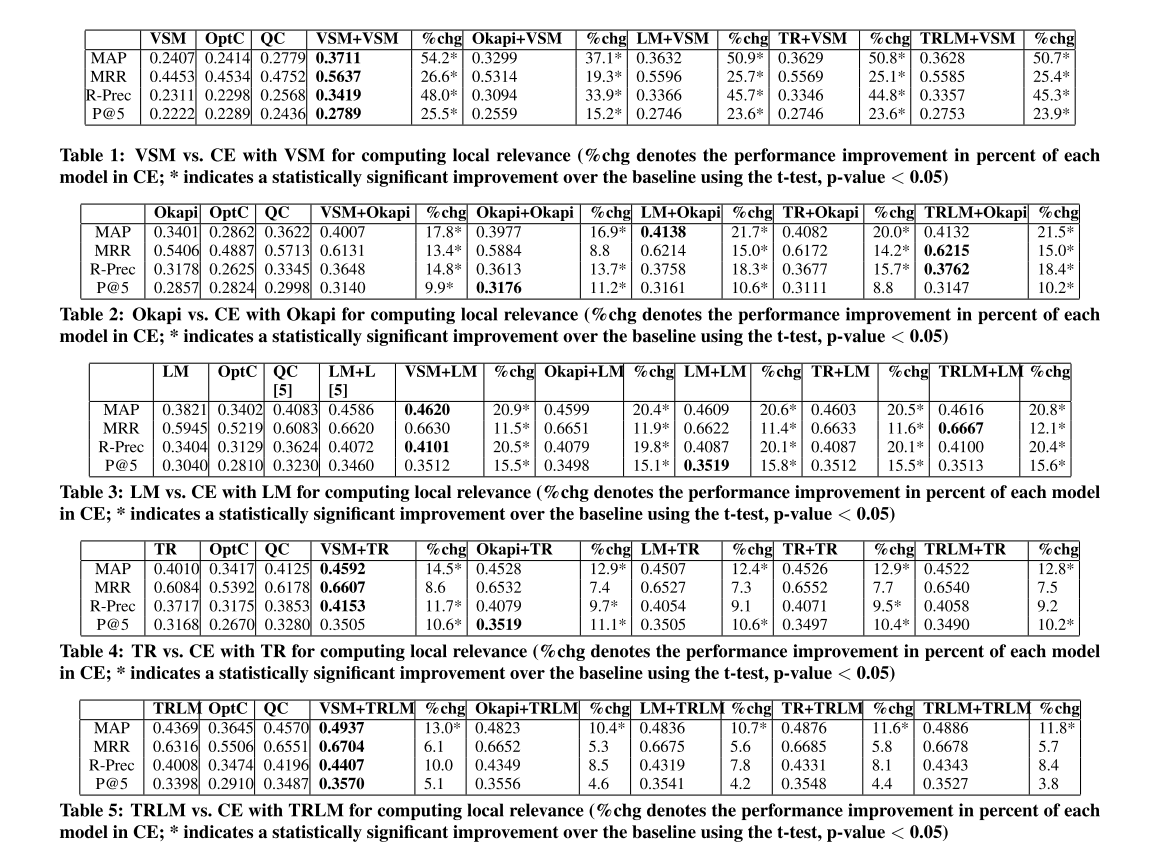
\includegraphics[height=6cm,width=10cm]{ana.png}
  \caption{Result Analysis}
  \label{fig:gr}
  \end{figure}
  
}

\frame{
  \frametitle{Result Analysis - Global Relevance}

  \begin{description}
  \item[TR and TRLM] 在计算全局相关度时,不如LM好,在baseline的情况,基于翻译的模型能够找到语义相同的不同词,但是在类内计算全局相关度时,在相关类别上,一般词表都差不多,减弱了语义不同词的影响。
    
  \end{description}

}

\section{MDL based model}

\subsection{intuition}

\frame{
  \frametitle{intuition}

  \begin{figure}
  \centering
  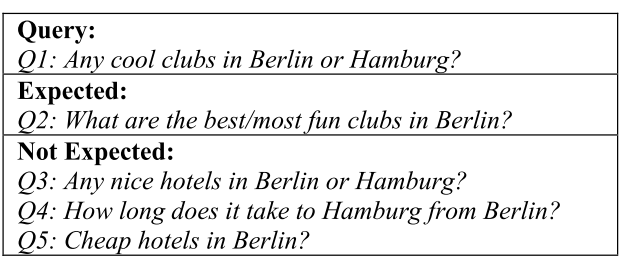
\includegraphics[height=4cm,width=8cm]{querysearch.png}
  \caption{intuition}
  \label{fig:gr}
  \end{figure}
}



\frame{
  \frametitle{intuition续}

  \begin{itemize}
  \item 对于问句 Any clubs in Berlin or Hamburg?
  \item 将问句分成两部分:
    \begin{description}
    \item[question topic] Berlin Hamburg
    \item[question focus] clubs
    \end{description}
  \item 在选词的时候,选定一些基本的词(BaseNP - Base Noun Phrase),和一些疑问词开头的句式(WH-ngram)。
  \end{itemize}
}

\subsection{Topic Chain}
\frame{
  \frametitle{Topic Chain}
  
  \begin{displaymath}
    p(c|t) = \frac{count(c,t)}{\sum_{c\in C} count(c,t)}
  \end{displaymath}
  对于词t和类别c。

  \textbf{specificity}

  \begin{displaymath}
    s(t) = \frac{1}{-\sum_{c\in C} p(c|t) \log (p(c|t)) + \epsilon}
  \end{displaymath}

  specificity 越大表明词的区分度越大。
}

\frame{
  \frametitle{构建topic chain}

  \begin{figure}
  \centering
  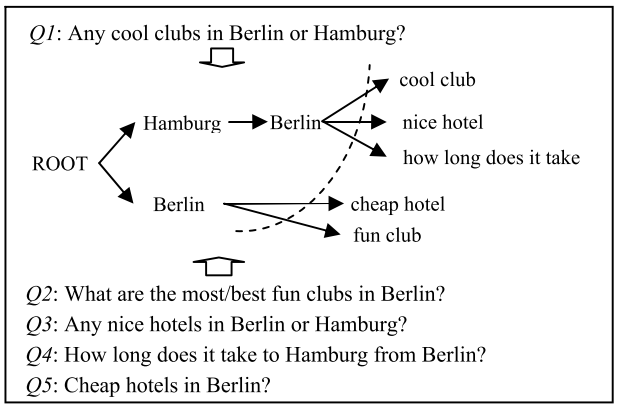
\includegraphics[height=4cm,width=6cm]{tree.png}
  \caption{question tree}
  \label{fig:gr}
  \end{figure}

}

\frame{
  \frametitle{tree cut}

  \begin{itemize}
  \item   通过tree cut的方式将问句q分成两部分:$H(q),T(q)$。
  \item H(q) 为 question topic
  \item T(q) 为 question focus
  \end{itemize}

}

\frame{
  \frametitle{检索}

  \begin{figure}
  \centering
  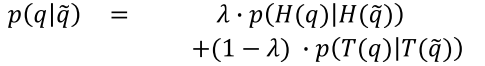
\includegraphics[height=1cm,width=6cm]{jiansuo1.png}
  \caption{检索}
  \label{fig:gr}
  \end{figure}

  \begin{figure}
  \centering
  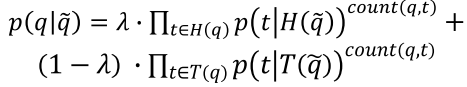
\includegraphics[height=1cm,width=6cm]{jiansuo2.png}
  \caption{检索}
  \label{fig:gr}
  \end{figure}
  
}

\subsection{结果}

\frame{
  \frametitle{Result}
  
  \begin{figure}
  \centering
  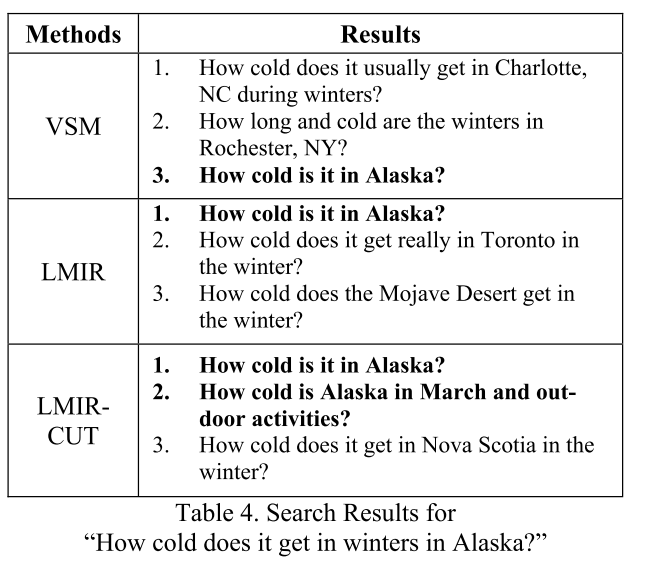
\includegraphics[height=6cm,width=6cm]{a1.png}
  \caption{检索结果}
  \label{fig:gr}
  \end{figure}
}

\frame{
  \frametitle{Result2}
  
  \begin{figure}
  \centering
  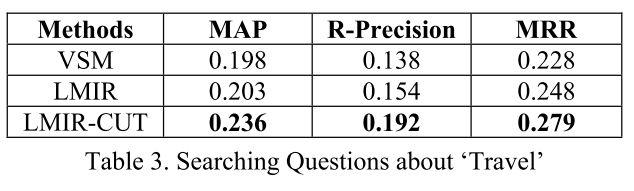
\includegraphics[height=2cm,width=5cm]{a2.png}
  \caption{检索结果}
  \label{fig:gr}
  \end{figure}

  \begin{figure}
  \centering
  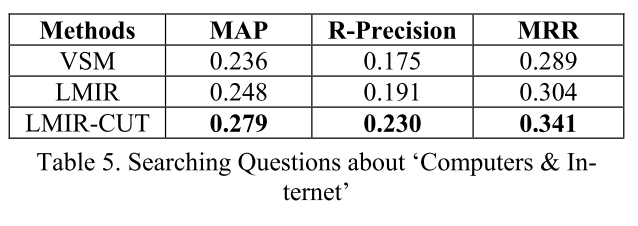
\includegraphics[height=2cm,width=5cm]{a3.png}
  \caption{检索结果}
  \label{fig:gr}
  \end{figure}

}

\frame{
  \frametitle{Topic Model based Method}

  \begin{figure}
  \centering
  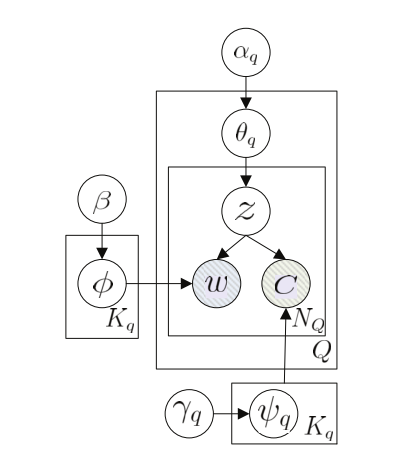
\includegraphics[height=6cm,width=6cm]{topicmodel.png}
  \caption{Topic Model}
  \label{fig:gr}
  \end{figure}

}

\frame{
  \frametitle{The end}
  
  Thanks!
}

\end{document}
